\begin{frame}[t]{Scope of Work}
	\topline
    \begin{itemize}
    	\item \textcolor{navy_theme}{\textbf{Indexing of Biometric Data}}
    	\vspace{1em}
			\begin{figure}[!ht]
				\centering 
				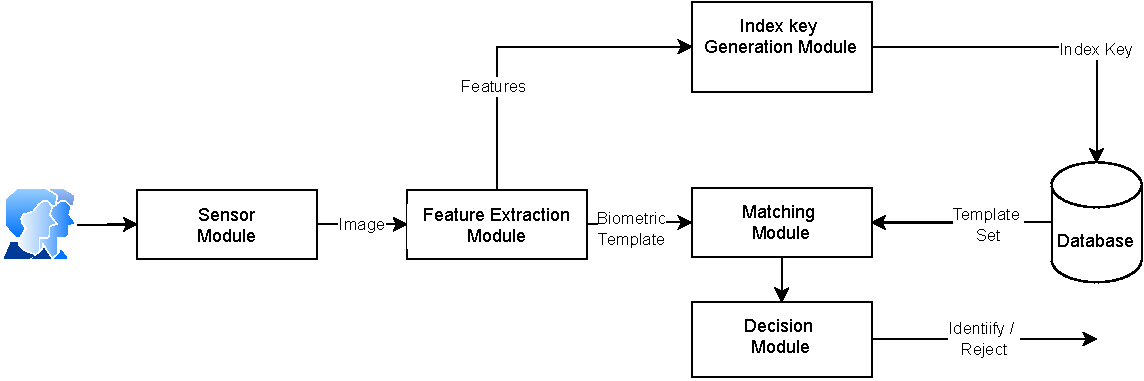
\includegraphics[width=0.90\textwidth]{images/steps_in_identification_with_indexing.drawio.pdf}
				\caption{Steps in Biometric Identification with indexing}
				\label{fig:bio_indexing2}
			\end{figure}
	\end{itemize}
\end{frame}


\begin{frame}[t]{Motivation}
	\topline
    \begin{itemize}
		\setbeamercovered{transparent}
    	\item<1> \textcolor{navy_theme}{\textbf{Limitations of Biometric Identification}}
		\vspace{1em}
		\begin{itemize}
			\setlength\itemsep{1em}

			\item False Matching

			\item Long Response Time
		\end{itemize}
		\vspace{1em}
		\invisible<1>{\item<2-> \textcolor{navy_theme}{\textbf{The Solution}}
		\vspace{1em}
		\begin{itemize}
			\setlength\itemsep{1em}

			\item Indexing

			\item Considering multiple biometric modalities
		\end{itemize}}
	\end{itemize}
\end{frame}


\begin{frame}[t]{Objectives}
	\topline
    \begin{itemize}
    	\item \textcolor{navy_theme}{\textbf{Research Objectives}}
		\vspace{1em}
		\begin{enumerate}
			\setlength\itemsep{1.5em}
			\setbeamercovered{transparent}
		    \item<1,5>{To create a large-scale virtual multi-modal biometric dataset and compare its performance on traditional indexing schemes and the proposed method.}

			\item<2,5>{ To design and implement an effective and scalable indexing scheme using Fingerprint as the biometric modality.}
			
			\item<3,5>{ To design and implement an effective and scalable indexing scheme using Iris as the biometric modality.}
			
			\item<4,5>{ To design and implement an effective and scalable indexing scheme in a multi-modal biometric system.}
		\end{enumerate}
	\end{itemize}
\end{frame}